\documentclass[12pt]{article}
\usepackage{geometry} 
\usepackage{graphicx}
\usepackage{float}
\usepackage{subcaption}
\usepackage{url}
\usepackage{mathtools}
\usepackage{color}
\usepackage{natbib}
\usepackage{fullpage}
\usepackage{amsmath}
\usepackage{amsfonts}
\usepackage{bigints}

% Make paragraphs not indented and leave a line between paragraphs
\setlength{\parskip}{\baselineskip}%
\setlength{\parindent}{0pt}%

\newcommand{\e}[1]{{\mathbb E}\left[ #1 \right]}
\newcommand{\gb}[1]{{\em \color{magenta} #1}}
\newcommand{\plr}[1]{{\em \color{green} #1}}
\newcommand{\gc}[1]{{\em \color{blue} #1}}

\geometry{a4paper}

\title{A Novel Spatial Framework for Understanding Genetic Admixture}
\date{\vspace{-5ex}}
\author{Gideon S. Bradburd$^{1,a}$, Peter L. Ralph$^{3,b}$, Graham M. Coop$^{1,c}$}

\begin{document}

\maketitle

\textsuperscript{1}Center for Population Biology, Department of Evolution and Ecology, University of California, Davis, CA 95616

\textsuperscript{3}Department of Molecular and Computational Biology, University of Southern California, Los Angeles, CA 90089

\textsuperscript{a}gbradburd@ucdavis.edu; 
\textsuperscript{b}pralph@usc.edu;
\textsuperscript{c}gmcoop@ucdavis.edu\\\\\

\newpage

\begin{abstract}
The patterns of genetic variation observed in modern populations are the product of a complex demographic and evolutionary history.  Genetic data can be used to illuminate that history, providing information about when and how populations have diverged, how migration connects populations, and how population sizes have fluctuated over time.  Work in this area has largely focused on estimating a population phylogeny, in which shared branch length on a tree represents shared evolutionary history between a pair of populations sampled in the modern day.  However, patterns of population differentiation are rarely tree-like, as migration and colonization will continuously re-shape patterns of relatedness between populations.  Isolation by distance (IBD), in which population differentiation increases with the distance between them, may offer a more natural null hypothesis.  Here, we present a novel analytical framework, SpaceMix, for the study of spatial genetic variation and genetic admixture, and a simple statistic to describe a population�s admixture status.
\end{abstract}

\newpage
%%%%%%%%% %%%%%%%%% %%%%%%%%%
\section*{Introduction}

Population-level demographic processes leave their mark on patterns of genetic variation and differentiation within and between populations.  Recent population genetics methods have focused on ways of learning about those processes from genetic observations, including demographic inference from the allele frequency spectrum (Song) and inference of the ancestral recombination graph from orthologous sequence data (Song, Rasmussen\&Siepel).  

Further work has focused on joint inference and visualization of whole-genome patterns of relatedness, specifically on estimating a population phylogeny describing the evolutionary history shared between sampled individuals or populations (e.g. Pickrell \& Pritchard, Patterson \& Moorjani, Reich?).  The approach of modeling relatedness between populations within species as a tree-like structure was pioneered by Cavalli-Sforza (\&Thompson?) in the 1960s \gb{?}, when genetic character data (blood types) were first becoming available in humans.  

Their work has been greatly extended by Pickrell and Pritchard (2012), whose method, TreeMix, models covariance in allele frequencies across loci as a directed acyclic graph between populations.  TreeMix then accommodates reticulate population structure by allowing branches on the population tree tree to be connected by arrows of admixture that explain excess residual covariance between populations or population 'clades.' 

In parallel, Patterson and Reich and Moorjani and Other Folks have developed a suite of tests for genetic admixture between a set of populations assuming a tree-like structure to their evolutionary history.  These tests model shared genetic drift as shared branch length on a hypothesized population tree, and take covariance in excess of that stipulated by the tree to be evidence for admixture.

These tree-based methods are both valuable as genetic inference and visualization tools.  However, a more natural framework for modeling genetic differentiation between sampled populations or individuals may be that of isolation by distance (IBD) (Wright).  The pattern of IBD, in which genetic differentiation increases with the geographic distance between populations, is ubiquitous in nature (Meirmans 2012, Ralph \& Coop 2012), and relies only on the weak assumption that individual's mating opportunities are geographically limited by dispersal.  

%Isolation by distance is, in many ways, a more reasonable null hypothesis of population relatedness than a population phylogeny;  \gb{too compare-y?  should I ditch this?} population structure will only rarely be truly tree-like, and a strictly bifurcating graph is unable to accommodate many geographic scenarios, such as multiple equidistant populations in migration-drift equilibrium.

Here, we present an analytical framework and develop an inference algorithm for studying the spatial distribution of genetic variation based on a model of isolation by distance.  We also introduce a simple statistic for quantifying a population's admixture status, and demonstrate the utility of this approach with two high profile empirical applications.

%%%%%%%%% %%%%%%%%% %%%%%%%%%
\section*{Methods}
Throughout these Methods, we will introduce example scenarios, simulated under a neutral, spatially structured coalescent process.  We will also present the results of SpaceMix analyses run on those data, both to illustrate its utility and clarify our presentation.  For all details of simulation procedure and analyses, please see Appendix X.

\subsection*{Data}
Our data consist of $L$ unlinked variable loci sampled across $K$ populations, as well as the geographic coordinates, denoted $G_k$, (latitude and longitude) at which those populations were sampled.  For convenience, we use bi-allelic single nucleotide polymorphisms (SNPs) as the genetic data in our descriptions below, but we note that this method could be applied equally well to other types of data, including microsatellites.  We refer to the $K$ accessions as populations, but the method can also be applied to individuals.  We summarize these genetic data as a set of allelic count data and sample size data, arbitrarily choosing an allele to count at each locus, and denoting the number of the counted allele at locus $\ell$ in population $k$ as $C_{\ell,k}$ out of a total sample size of $S_{\ell,k}$ alleles.  The sample frequency of the counted allele at locus $\ell$ in population $k$ is therefore $\hat{f}_{\ell,k} = C_{\ell,k}/S_{\ell,k}$.  Our method models the covariance in these allele frequencies between populations across loci.


%%%%%%%%% %%%%%%%%% 
\subsection*{The Normal Approximation to Drift}
In order to model this covariance, we draw on previous work (Cavalli-Sforza \& Edwards, Nicholson et al 2002, Coop et al 2010, Pickrell \& Pritchard 2012), and model the process of genetic drift as approximately Gaussian.  Briefly, if the frequency of allele $\epsilon$ in an ancestral population, $A$ is $\epsilon_A$, then we model the frequency of that allele in a daughter population,  $B$, as follows:
\begin{equation}
\label{eq:normal_drift}
\epsilon_B \sim N(\epsilon_A,\delta_B(\epsilon_A)(1-\epsilon_A))
\end{equation}
The parameter $\delta_B$, the amount of drift that has occurred in $B$ since it split off from $A$, is approximately equal to $\frac{t}{2N_e}$, where $t$ is time in generations, and $N_e$ is the effective population size.  Note that the binomial variance term in the normal variance in \eqref{eq:normal_drift} ignores the fact that the drift variance will change from generation to generation due to changes in the frequency of $\epsilon$ within a population over time.  Note also that this approximation works best for alleles at intermediate frequency, which are less likely to be lost or fixed during the interval separating $A$ and $B$.  However, if the extent of drift sufficiently limited (time scales are short or population sizes are large), the approximation of inter-generational binomial sampling to Brownian motion is good (\gb{see figure comparing fit of binomial sampling to fit of normal approx?}).  

Between populations, the differentiating process of drift is counteracted by the homogenizing force of migration, so that populations with higher levels of historical or ongoing migration can be thought of as having more shared drift.  Across loci, populations with highly shared drift will tend to covary more strongly in the deviations their allele frequencies take from some ancestral (or global) mean.

%%%%%%%%% %%%%%%%%% 
\subsection*{Mean-centering and normalizing variance}
The multivariate normal distribution offers a natural statistical framework for describing this covariance, which may be straightforwardly modeled as a parametric function of any pairwise variable (see, e.g., Bradburd, Ralph, and Coop 2013).  Unlike multivariate normal observations however, allele frequencies at variable loci are constrained to have a mean between 0 and 1, and may have heterogeneous variance across loci.  To more closely meet the assumptions of our statistical inference model, we mean-center and normalize our observations by the following procedure.

Recall that the sample allele frequency at locus $\ell$ in population $k$ is given by $\hat{f}_{\ell,k} = C_{\ell,k}/S_{\ell,k}$.  We wish to calculate a sample mean frequency at each locus weighted by the sample size in each population.  As sample size may vary across loci, we first calculate $\bar{S}_k$, the mean population sample size in population $k$, as $\bar{S}_k = \frac{1}{\ell}\sum_\ell S_{\ell,k}$.  We then calculate the weighted sample mean frequency at locus $\ell$ as follows:
\begin{equation}
\label{eq:sample_mean_freq}
\bar{f}_{\ell} = \frac{1}{\sum_k S_{\ell,k}} \sum_k \hat{f}_{\ell,k} S_{\ell,k}
\end{equation}
The binomial variance at each locus varies as a function of the global allele frequency, and, at locus $\ell$, is given by $\bar{f}_{\ell}(1-\bar{f}_{\ell})$.  To avoid modeling the heterogeneous effect of this variance across loci, we standardize by the binomial variance.  We call the mean-centered normalized allele frequencies $X_{\ell,k}$, and calculate them as follows:
\begin{equation}
\label{eq:MCN_freqs}
X_{\ell,k} = \frac{ \hat{f}_{\ell,k} - \bar{f}_{\ell} } {\bar{f}_{\ell}(1-\bar{f}_{\ell})}
\end{equation}
We then model these transformed data as multivariate normal, as described in the next section.  Note, by using the sample mean frequency to mean-center our observations, we lose a degree of freedom, and can also induce negative covariance across loci between populations.  We discuss this further in Appendix A.

%%%%%%%%% %%%%%%%%% 
\subsection*{Spatial Covariance Model}

We wish to model the covariance between populations as the result of a spatial process, in which migration rates between nearby populations are higher than between distant ones, so that a population has higher covariance with a close neighbor than with a more distant population.  The form of our parametric covariance matrix fits a model of exponential decay to allele frequency covariance with geographic distance (Wasser et al 2004, Bradburd, Ralph, and Coop 2013).  The covariance between populations $i$ and $j$ is 
\begin{equation}
\label{eq:spatial_covariance}
\omega_{i,j} = \frac{1}{\alpha_0} \text{exp} \left(	\left( \alpha_1D_{i,j} \right)^{\alpha_2} \right)\text{,}
\end{equation}
where $D_{i,j}$ is the geographic distance between population $i$ and $j$ (and therefore a function of their locations, $G_i$ and $G_j$), $\alpha_0$ controls the sill of the covariance (the within-population variance, or the covariance when distance between points is 0),  $\alpha_1$ controls the rate of the decay of covariance per unit pairwise distance, and $\alpha_2$ determines the shape of that decay.
We model the sample covariance of mean-centered normalized allele frequencies ($Y$) as Wishart with degrees of freedom equal to the number of loci ($L$) across which the covariance is calculated.
That is, 
\begin{equation}
\label{eq:wishart_dist}
Y \sim \mathcal{W}\left( L^{-1} \omega, L	\right)
\end{equation}


The likelihood of the data $X_{\ell,k}$, given the observed distance matrix $D$ between all $K$ populations and the values of the three $\alpha$ parameters ($\vec{\alpha}$), which together parameterize the spatial covariance matrix $\omega$, is given by
\begin{equation}
\label{eq:wishart_lnl}
\mathcal{P}(X_{\ell,k} \; | \; D(G), \pmb{\vec{\alpha}}) = \frac{|Y|^{ \frac{L - K - 1}{2} } \text{exp} \left(  \frac{-\text{tr}(\pmb{\omega}^{-1}Y)}{2}	\right) }	
									{2^{\frac{LK}{2}}  |\frac{\pmb{\omega}}{L}|^{\frac{L}{2}}  \Gamma_{p}\!\left(  \frac{L}{2} \right)	},
\end{equation}
where $\text{tr}$ denotes the trace function and $\Gamma_p$ denotes a multivariate gamma function, and all boldface variables are parameters estimated as part of our inference procedure.


%%%%%%%%% %%%%%%%%% 
\subsection*{Accommodating non-equilibrium processes}
%\gb{MS simulation of pops on a grid, figure to show that we recover the grid}
%\gb{MS simulation of pops on a grid with a barrier in the middle, figure to show how pops on either side of barrier clump together (or how pops scuttle away from each other)}

\gb{MS simulation of pops on a grid with a recent expansion, figure to show how those pops all clump toward source of expansion}

This model assumes that the system is in migration-drift equilibrium and that every unit of pairwise geographic distance is equivalent in its contribution to decay of allelic covariance, but in many cases those assumptions will not be met.

Non-equilibrium processes like long distance dispersal, recent migration, colonization, or population expansion events will distort the shape of the decay of covariance with distance, and may bias parameter estimation.  Depending on the distribution and history of these events over the landscape, they may also result in heterogeneous patterns of the decay of covariance over space.  Strong barriers to dispersal on the landscape can also bias the estimation of the contribution of a unit distance to decay in covariance.

To accommodate these heterogeneous processes, we can treat population's locations on the landscape as a random variable, and estimate them as part of our inference procedure.  Two populations that are sampled at distant locations but that are genetically similar (perhaps one was recently founded by a colonization event from the other) may choose estimated locations that are nearby, while two populations that are sampled close together, but that are genetically dissimilar (e.g, the recently founded population and its neighbor), may choose locations that are farther apart.
The result is a map \gb{how do we feel about the word "geogenetic?"} in which the distances between populations are indicative of the way that populations perceive the distances between themselves.  There is a rich history of this type of data visualization, especially using reduced dimensionality representations of the data such as Principal Components Analysis (e.g. Menozzi, Piazza, and Cavalli-Sforza 1978, Novembre et al 2008, Novembre and Stephens 2008).  Our method offers an improvement over PCA-based visualization methods in that it offers an explicit model of spatial genetic variation, and can therefore be used as a robust framework for inference and hypothesis testing (see also Yang et al 2012, Yang et al 2014).

Our likelihood function is now given by,
\begin{equation}
\label{eq:choose_location_wishart_lnl}
\mathcal{P}(X_{\ell,k} \; | \; \pmb{D}(\pmb{G'}), \pmb{\vec{\alpha}}) = \frac{|Y|^{ \frac{L - K - 1}{2} } \text{exp} \left(  \frac{-\text{tr}(\pmb{\omega}^{-1}Y)}{2}	\right) }	
									{2^{\frac{LK}{2}}  |\frac{\pmb{\omega}}{L}|^{\frac{L}{2}}  \Gamma_{p}\!\left(  \frac{L}{2} \right)	},
\end{equation}
where $\text{tr}$ denotes the trace function and $\Gamma_p$ denotes a multivariate gamma function, and all boldface variables are parameters estimated as part of our inference procedure.  Notice that this equation has the same form as \eqref{eq:wishart_lnl}, save that the pairwise geographic distance matrix $D$ is now a parameter to be estimated rather than an observed value.

We use the observed location for population $k$, $G_k$, to parameterize a bivariate normal spatial prior on the location $k$ chooses for itself, $G'_k$ (for more details on our Bayesian inference procedure, see Appendix B).  However, we can use random locations as the ``observed locations" ($G_k$) can remove any influence of the observed map on the output via the prior, or we can change the variance on the spatial priors to ascertain the effect of the prior on inference.

To illustrate this inference procedure, we present several simulated scenarios, featured in Figure \ref{sfig:lattice_scenarios}, as well as the output of SpaceMix analyses run on them.  In the first scenario (Fig. \ref{sfig:lattice_scenarios}\subref{lattice_pops}), we simulate populations on a lattice, with symmetric nearest neighbor migration (attenuated by $\sqrt{2}$ on the diagonals).  In our second scenario (Fig. \ref{sfig:lattice_scenarios}\subref{barrier_pops}), we simulate under the same lattice scenario, but introduce a barrier to dispersal, across which migration rates are attenuated by a factor of 5.  On both scenarios, we perform SpaceMix analyses in which we treat population locations as random variables to be estimated as part of the model, and randomly place the `observed' location of each population on a line so as to remove the influence of the prior.

\begin{figure}
	\centering
		\subcaptionbox{Populations on a lattice \label{lattice_pops}}
			{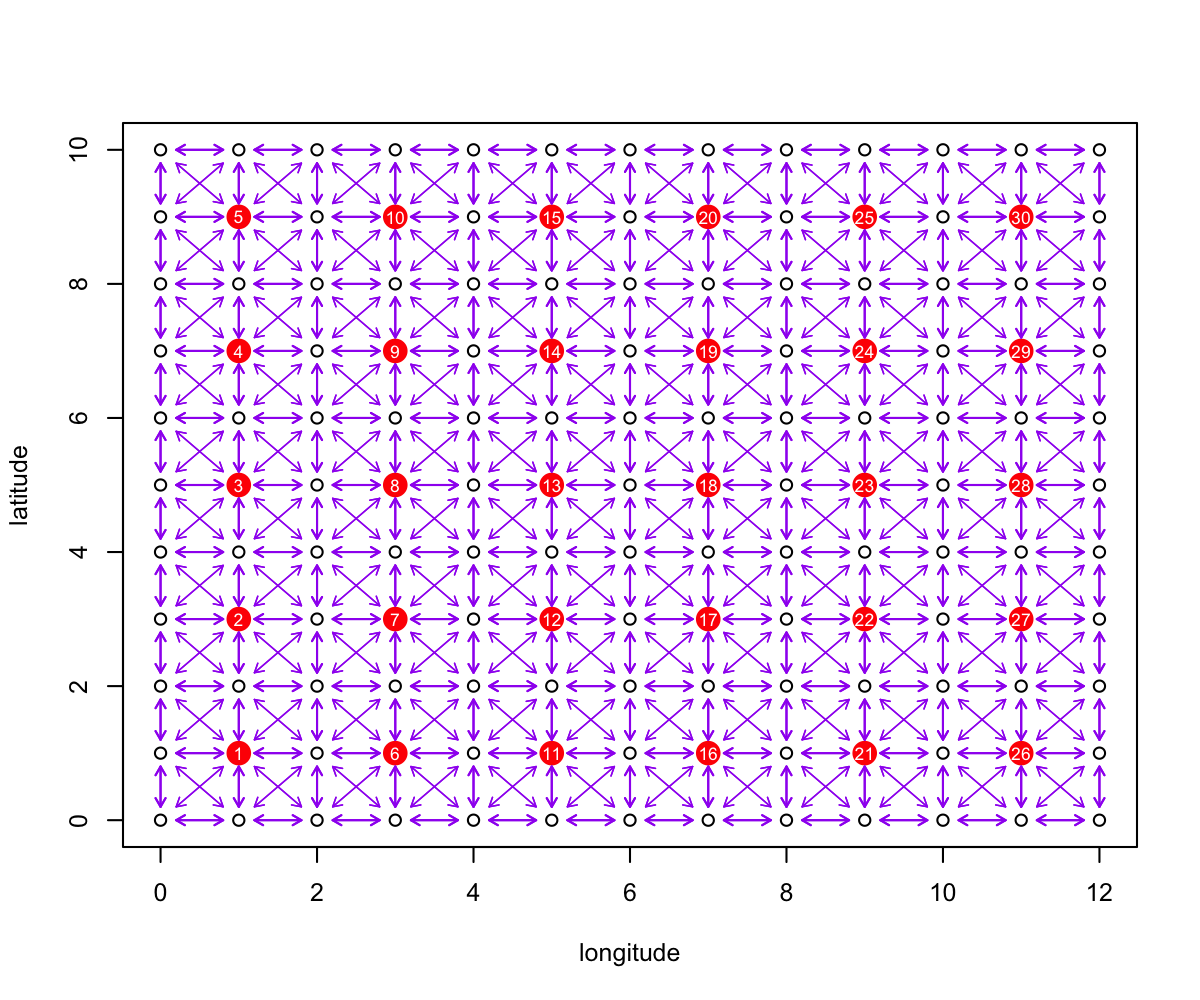
\includegraphics[width=2.4in,height=2in]{stationary_pops_map.png}}
		\subcaptionbox{SpaceMix map \label{lattice_pops_inference}}
			{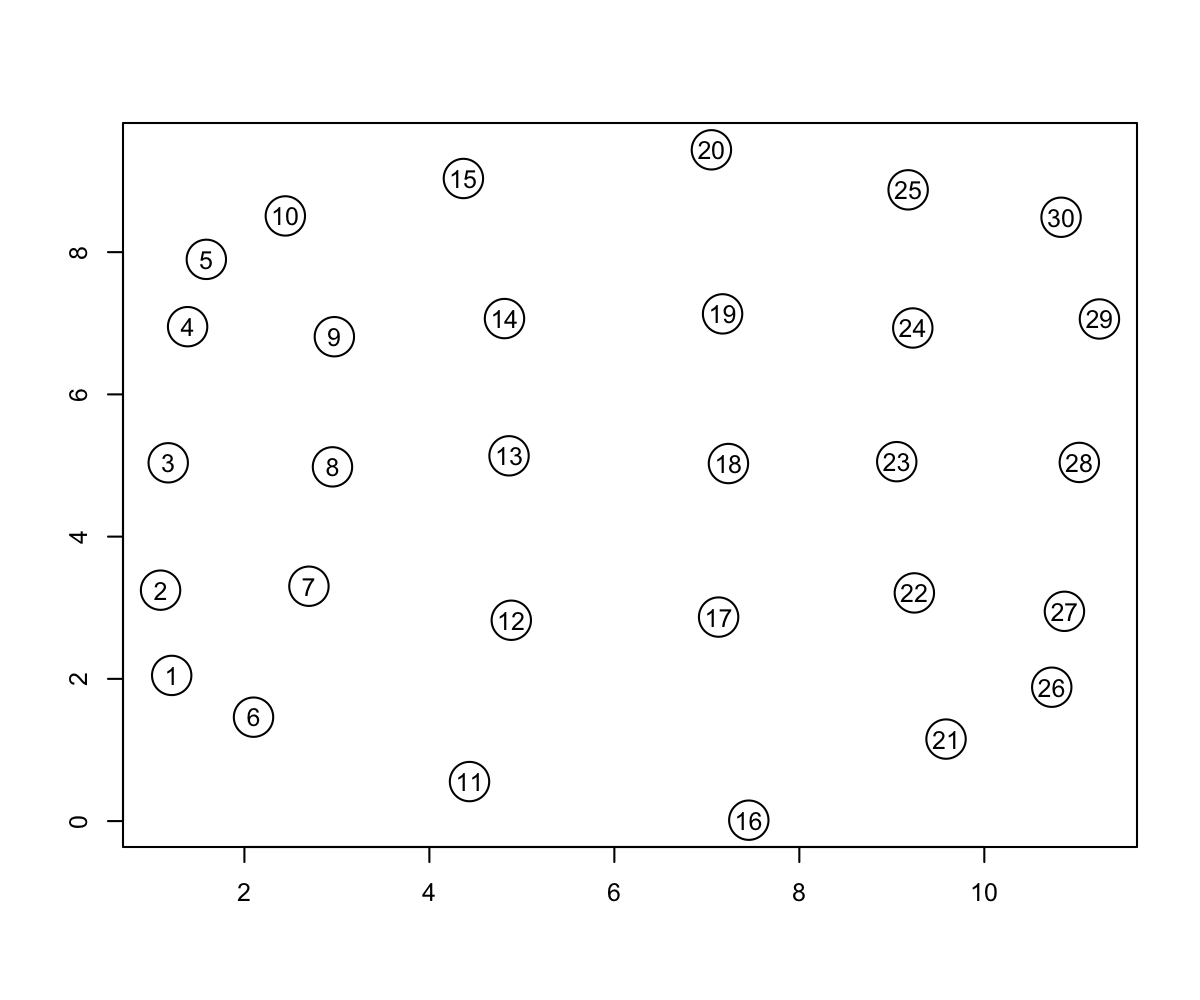
\includegraphics[width=2.4in,height=2in]{stationary_pops_1_inference_map.png}}
		\subcaptionbox{A lattice with a barrier \label{barrier_pops}}
			{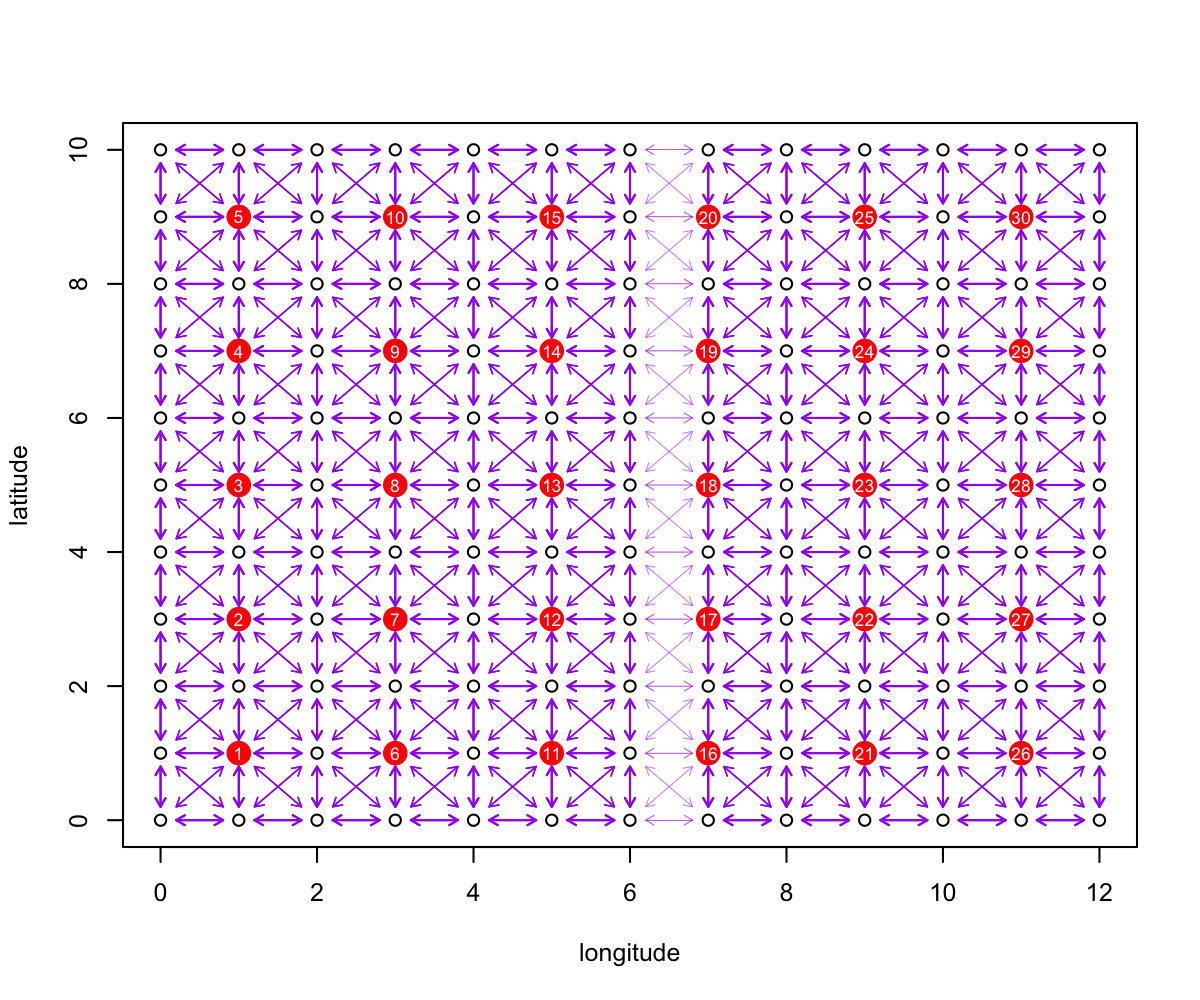
\includegraphics[width=2.4in,height=2in]{barrier_map.png}}
		\subcaptionbox{SpaceMix map \label{barrier_pops_inference}}
			{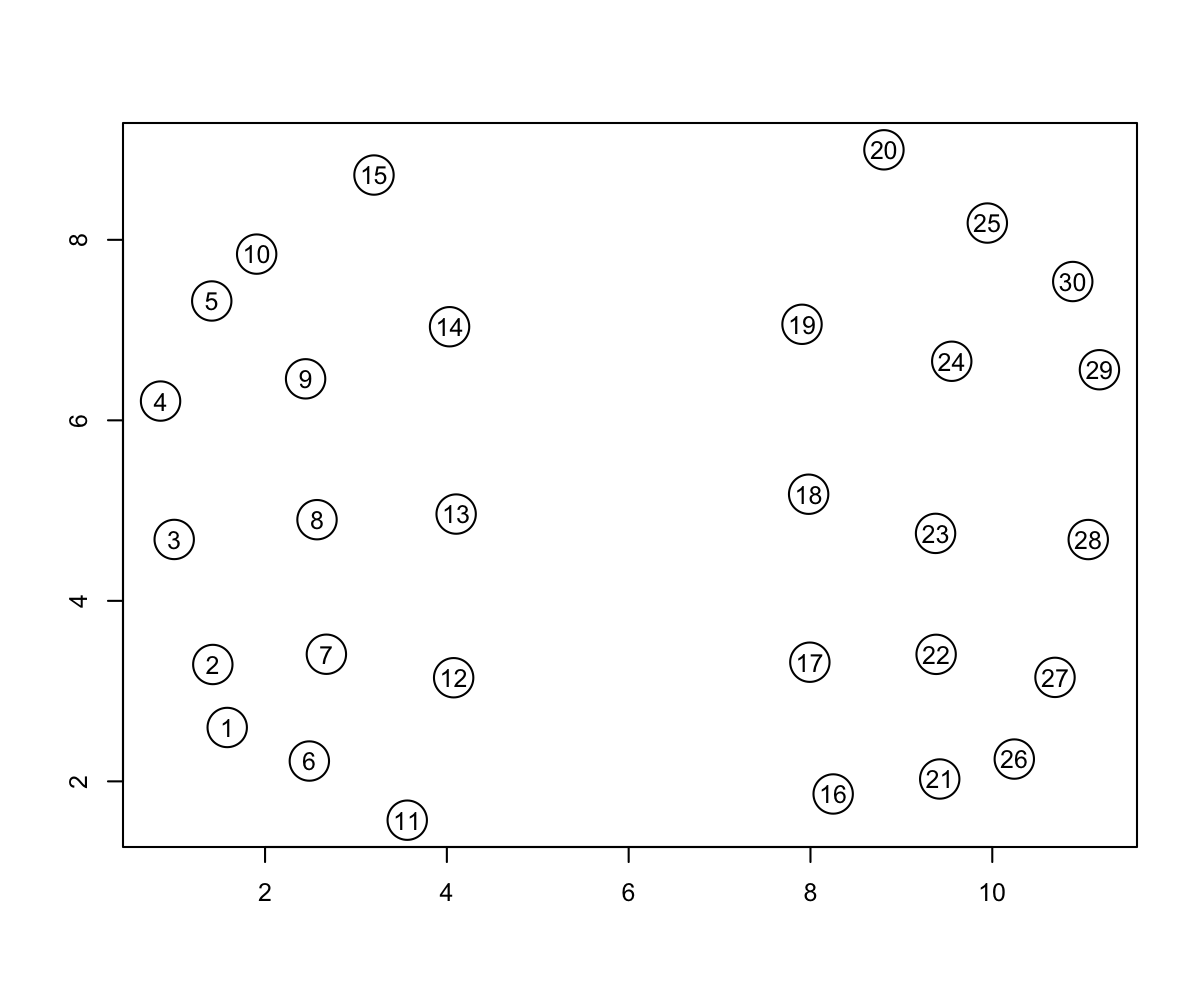
\includegraphics[width=2.4in,height=2in]{barrier_1_inference_map.png}}
	\caption{Simulated scenarios and the corresponding population maps inferred using SpaceMix.  For clarity of presentation, the inferred coordinates have have been Procrustes transformed around the coordinates of the lattice used to simulate the data.}\label{sfig:lattice_scenarios}
\end{figure}

In Figure \ref{sfig:lattice_scenarios}\subref{lattice_pops_inference}, the reader can see that the configuration estimated for the populations by SpaceMix matches the lattice structure used to simulate the data, and that populations are correctly choosing their nearest neighbors.  Similarly, in Figure \ref{sfig:lattice_scenarios}\subref{barrier_pops_inference}, the population configuration matches that of the lattice used to simulate the data, but the reader can see that, due to the influence of the barrier, the two halves of the map have pushed farther away from one another.  This gap between populations on either side of the barrier reflects the way those populations perceive the distance between them.

%%%%%%%%% %%%%%%%%% 
\subsection*{Spatial Admixture Statistic}
\gb{Figure 2: MS simulation of pops on a grid with 1 admixture event from a pop on one side to a pop on the other}

\gb{3a figure to show the pairwise f-stat between all pops and the admixed pop}

\gb{3b figure to show landscape of admixture to the admixed pop}

\gb{close with figure 4: what the choose your own locations do with the admixture}
Given a model of isolation by distance and allele frequencies sampled at different points on a map, we can calculate (1) whether a population's genetic makeup is well predicted by that of its neighbors, and (2) whether a focal population has excess covariance with another sampled population or unsampled region of the map.  These statistics, which we call spatial $f$-statistics \gb{should we give these a real name?}, are in the spirit of both the $f_n$ statistics introduced by Reich et al (2009) and the admixture arrows in a TreeMix graph (Pickrell and Pritchard 2012), and are designed to pick up the signal of covariance between populations in excess of that predicted by the model.  Where both those approaches use a model of a population phylogeny, ours uses a spatial model of allelic covariance, in which one population's covariance with another is expected to decay at a fixed manner across the landscape, as determined by the estimated parametric form of the spatial covariance.  The details of this procedure are given below, and illustrated with a simulated example scenario (see Figure \ref{sfig:admixture_scenario}), featuring an admixture event.

\begin{figure}
	\centering
	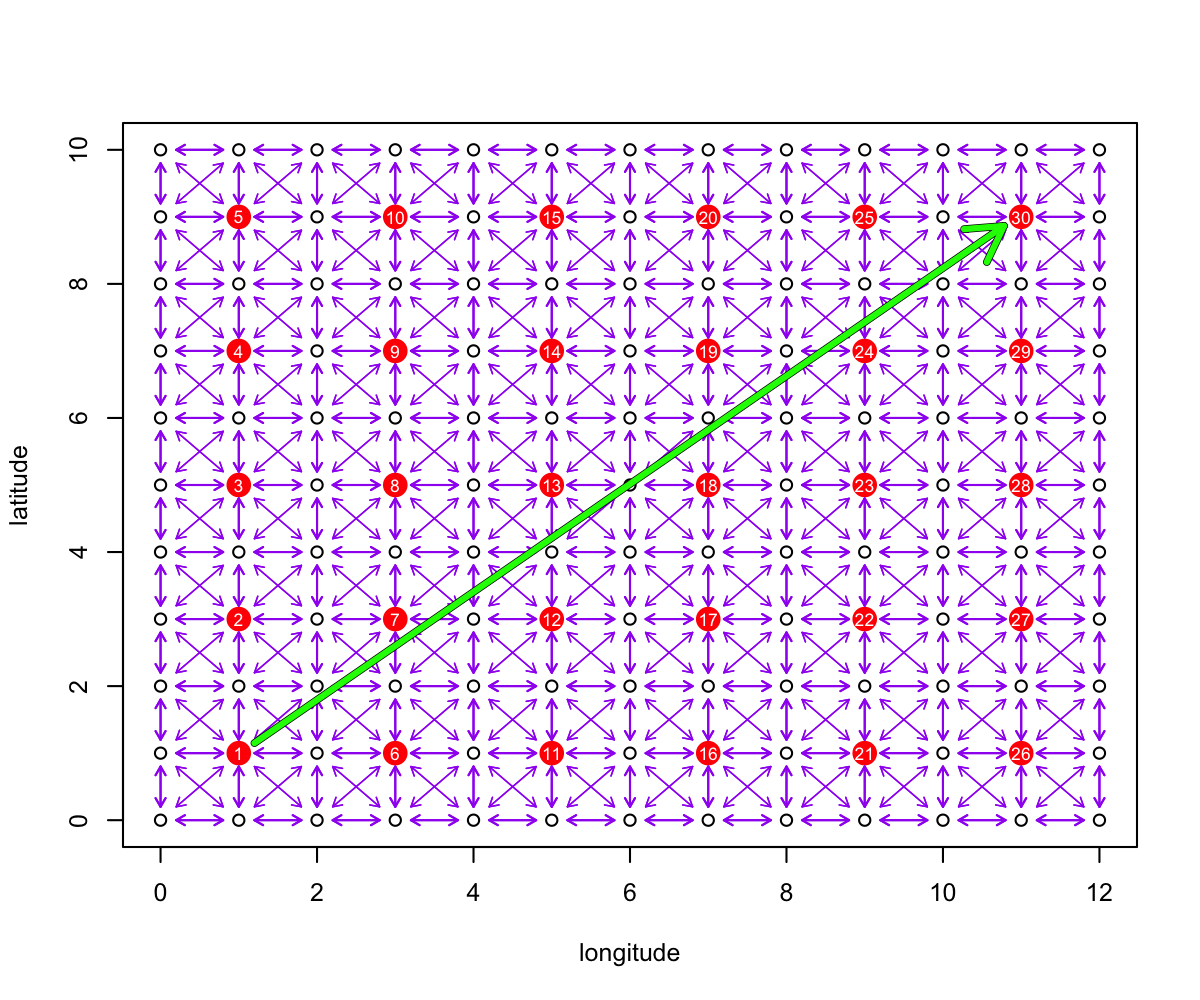
\includegraphics[width=2.4in,height=2in]{admixture_map.png}
	\caption{In this simulated scenario, one population sampled in the modern day (Population 30) has had half of its population replaced with lineages from a distant population (Population 1), simulating an admixture event.}\label{sfig:admixture_scenario}
\end{figure}

Given a focal population $i$, the parametric spatial covariance matrix $\omega$, and the mean-centered, normalized allele frequencies $X$ at all sampled geographic locations $G$, we calculate the conditional mean observations $X$ at locus $\ell$ at location $G_i$ as
\begin{equation}
\label{eq:conditional_mean}
\bar{X}_i = \left(	\omega_{i,-i} \right) \left( \omega^{-1}_{-i,-i} \right) \left( X_{-i} \right),
\end{equation}
where we denote dropping the focal population $i$ from the covariance matrix or the observations $X$ at locus $\ell$ with a ``$-i$'' in the subscript.

Then, given the conditional mean observations in focal population $i$, $\bar{X}_i$, and a population $j$ with which we wish to test for admixture with $i$, we calculate our spatial admixture statistic over all $L$ loci as follows:
\begin{equation}
\label{eq:spatial_fstat_pop}
f_{i,j} = \frac{	\mathbb E_L\left[(\vec{X}_i- \bar{X}_i) ~ (\vec{X}_{j})\right]		}
			{\sqrt{	\text{Var}( \vec{X}_i- \bar{X}_i )  \text{Var}( \vec{X}_{j} )  }  }
\end{equation}

This statistic calculates whether a focal population's deviations from its spatial predictions have excess covariance with another sampled population.  It's significance can be assessed via a non-parametric bootstrap \gb{or jackknife???} across loci in the dataset.  \gb{Figure 3a shows the spatial \emph{f}-stat calculated between the admixed population and each other population.}

This statistic may also be calculated between a focal population $i$ and an arbitrary location $j'$ on the map.  First, we calculate the spatial covariance between all the arbitrary location $j'$ and the sampled populations, \emph{excluding} the focal population $i$.  This spatial covariance matrix, which we denote $\omega'$, therefore has rank $k$, as we have excluded the focal population $i$ and included the putative source of admixture location $j'$.  Next, we calculate the conditional mean observations $X_{j'}$ at locus $\ell$ at location $G_{j'}$ as follows:
\begin{equation}
\label{eq:conditional_mean}
\bar{X}_{j'} = \left(	\omega'_{-j',-j'} \right) \left( \omega'^{-1}_{-j',-j'} \right) \left( X_{-i} \right)
\end{equation}

Finally, we can calculate a spatial $f$-statistic between the focal population and the putative location from which it receives admixture as follows,
\begin{equation}
\label{eq:spatial_fstat_location}
f_{i,j'} = \frac{	\mathbb E_L\left[(\vec{X}_i- \bar{X}_i) ~ (\vec{\bar{X}}_{j'})\right]	}
			{\sqrt{	\text{Var}( \vec{X}_i- \bar{X}_i )  \text{Var}( \vec{\bar{X}}_{j'} )  }  }
\end{equation}

This procedure allows us to visualize the signature of excess covariance across the entire map. \gb{Figure 3b shows the spatial \emph{f}-stat calculated between the admixed population and each other population.}

%%%%%%%%% %%%%%%%%% 
\subsection*{Inference of Spatial Admixture}

This signal of excess covariance over anomalously long distances can be difficult to accommodate within the framework described above, in which we estimate the 2-dimensional configuration of populations that, along with a model of the decay of covariance in allele frequencies with distance, best describes their empirical patterns of genetic differentiation.  In Figure \ref{sfig:admixture_inference}, the reader can see the torturous lengths to which the method goes to come up with a configuration of populations that accommodates their genetic relationships.  The admixed population 30 is estimated to have a location intermediate between population 1, the source of its admixture, and populations 24, 25, and 29, the nearest neighbors to the location of its non-admixed lineages.  However, this warping of space is difficult to interpret, and does not have great utility for the visualization of genetic relationships.

\begin{figure}[ht!]
	\centering
	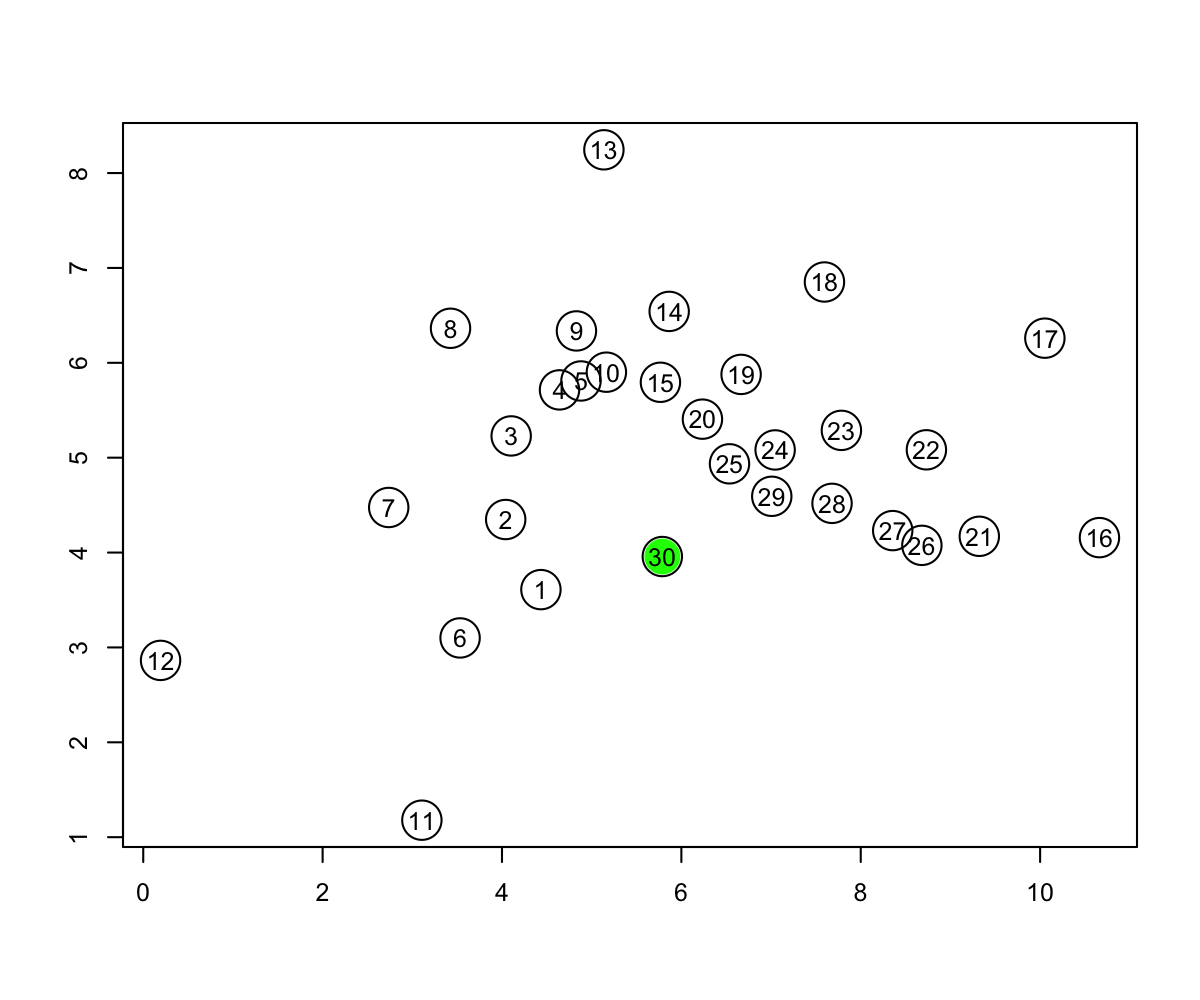
\includegraphics[width=2.4in,height=2in]{admixture_1_inference_map.png}
	\caption{Inference of population locations in the scenario depicted in Figure \ref{sfig:admixture_scenario}.  Population 30 has received half of its lineages from population 1, to simulate a long distance admixture event in the very recent past.}\label{sfig:admixture_inference}
\end{figure}

\gb{figure to show inference of admixture arrows}

Instead, we can interpret this excess covariance over anomalously long distances as genetic admixture, and we can incorporate it directly into out inference framework.  We define the allele frequency at locus $\ell$ in admixed population $k$ to be
\begin{equation}
f_{\ell,k} = pf_{\ell,i} + (1-p)f_{\ell,j},
\end{equation}
where $f_{\ell,i}$ is the allele frequency in population $i$, $f_{\ell,j}$ is the allele frequency in population $j$, and $p$ is the admixture proportion, which varies between 0 and 1 and describes the extent to which populations $i$ and $j$ are contributing to the genetic make-up of population $k$.

To infer the spatial context of this admixture, we allow each population a point in space (\gb{can I use the phrase `ghost population,' or is that too goofy?}) from which it draws its admixture, and we model both the location of that point and the extent (proportion) of that admixture.  The observed allele frequencies in sampled populations are therefore a weighted average of the model-estimated allele frequencies at the geographic location of the sampled population and those at the coordinates from which the observed population draws admixture.  That is, the observed allele frequencies in population $k$ are modeled as follows:
\begin{equation}
f_{k} = pf_{k'} + (1-p)f_{j},
\end{equation}
where $f_{k'}$ are the model-estimated allele frequencies across loci at the spatial location of population $k$ and $f_{j}$ are the model-estimated allele frequencies at the spatial location $j$ from which population $k$ is drawing admixture in proportion $p$.  The admixture proportion $p$ is constrained to vary between 0 and 0.5, such that at least half of a population's genetic make-up must be determined by its geographic location.

The covariance between sampled populations $i$ and $j$ can be modeled as
\begin{alignat}{3}
\label{eq:admixed_covariance_1}
\Omega_{i,j} = (1-p_i)(1-p_j) \omega_{i\;,\;j\;} \; \times&\\
(p_i)(1-p_j) \omega_{i',\;j\;} \; \times   \notag&\\
(p_j)(1-p_i) \omega_{i\;,\;j'} \; \times   \notag&\\
(p_i)(p_j) \omega_{i',\;j'} \; \phantom{\times}   \notag&
\end{alignat}
where $i'$ and $j'$ are the points from which populations $i$ and $j$ are drawing their admixture with proportions $p_i$ and $p_j$, and $\omega$ is the spatial covariance function parameterized by the pairwise geographic distances between each pair of populations.
In addition, we introduce a population-specific variance term on each diagonal element of the covariance matrix.  This term accommodates both the binomial sampling noise introduced by finite chromosome sample size in each population and also population-specific drift.  The full expression for our admixed covariance function is below.
\begin{alignat}{3}
\label{eq:admixed_covariance_2}
\Omega_{i,j} = (1-p_i)(1-p_j) \omega_{i\;,\;j\;} \; \times&\\
(p_i)(1-p_j) \omega_{i',\;j\;} \; \times   \notag&\\
(p_j)(1-p_i) \omega_{i\;,\;j'} \; \times   \notag&\\
(p_i)(p_j) \omega_{i',\;j'} \; +   \notag&\\
I\bar{S_k}^{-1} + \eta_k \phantom{+} \notag&
\end{alignat}

where $I$ is the identity matrix, $\bar{S_k}$ is the mean sample size in population $k$ across all loci, and $\eta_k$ is the nugget estimated in population $k$.

The location from which sampled population $k$ draws its admixture, $G_{k'}$, and the population's admixture proportion, $p_k$, are treated as random variables and jointly estimated as part of our inference procedure.  The admixed covariance between populations $i$ and $j$, $\Omega_{i,j}$ is then a function of all the pairwise spatial covariances between populations $i$ and $j$ and the points from which they draw admixture, $i'$ and $j'$.  Those spatial covariances in turn are a function of all combinations of pairwise distances between their locations: $G_i$, $G_i$, $G_{i'}$, and $G_{j'}$.

The likelihood function for this model in which each population is allowed to draw admixture from a point in space is 
\begin{equation}
\label{eq:choose_admixture_wishart_lnl}
\mathcal{P}\left(X_{\ell,k} \; | \; \pmb{D}\left(G,\pmb{G_{'}}\right), \pmb{\vec{\alpha}}, \pmb{p}, S, \pmb{\eta}\right) = \frac{|Y|^{ \frac{L - K - 1}{2} } \text{exp} \left(  \frac{-\text{tr}(\pmb{\Omega}^{-1}Y)}{2}	\right) }	
									{2^{\frac{LK}{2}}  |\frac{\pmb{\Omega}}{L}|^{\frac{L}{2}}  \Gamma_{p}\!\left(  \frac{L}{2} \right)	},
\end{equation}
where $\text{tr}$ denotes the trace function and $\Gamma_p$ denotes a multivariate gamma function, and all boldface variables are parameters estimated as part of our inference procedure.


For details on our Bayesian inference framework and Markov chain Monte Carlo inference procedure, please see the Section: How I spent the past year!

\subsection*{Models}
The models described above may be used in various combinations.  In the simplest model, populations may not choose their own locations, nor are they allowed to draw admixture, and the only parameters to be estimated are those of the spatial covariance function given in Eqn \eqref{eq:spatial_covariance}, and the population-specific variance terms ($\eta_k$).  In the most complex model, population locations, the locations of their sources of admixture, and the proportions of that admixture are all estimated jointly in addition to the parameters of the spatial covariance function and the population specific variances.  The full likelihood of this most complex parameterization is given by,
\begin{equation}
\label{eq:source_and_target_wishart_lnl}
\mathcal{P}\left(X_{\ell,k} \; | \; \pmb{D}\left(\pmb{G'},\pmb{G_{'}}\right), \pmb{\vec{\alpha}}, \pmb{p}, S, \pmb{\eta}\right) = \frac{|Y|^{ \frac{L - K - 1}{2} } \text{exp} \left(  \frac{-\text{tr}(\pmb{\Omega}^{-1}Y)}{2}	\right) }	
									{2^{\frac{LK}{2}}  |\frac{\pmb{\Omega}}{L}|^{\frac{L}{2}}  \Gamma_{p}\!\left(  \frac{L}{2} \right)	},
\end{equation}


\gb{A note about here how this complex model is still identifiable}

\section*{Empirical Applications}
To demonstrate the applications of this novel method, we employed it in two canonical empirical systems: the greenish warbler ring species complex, and, to our knowledge, the most complete geographic sampling of human populations to date (\gb{is this true?}).

\subsection*{Greenish Warblers}
Description of the data

Description of the research questions we use SpaceMix to address

Details of analyses run
\subsection*{Human Populations}
Description of the data

Description of the research questions we use SpaceMix to address

Details of analyses run

%%%%%%%%% %%%%%%%%% 
\section*{Results}
\gb{should we just merge the results section in with the empirical applications section?  not sure what else would go here.}

%%%%%%%%% %%%%%%%%% 
\section*{Discussion}
In this paper we have presented blah blah blah.  We believe this represents an advance over previous methods because blah blah blah.  This method can be used to answer a variety of empirical questions, including blah, blah, and blah, and also serves as an intuitive data visualization tool.

%%%%%%%%% %%%%%%%%% 
\subsection*{Empirical Results}

%%%%%%%%% %%%%%%%%% 
\subsubsection*{Greenish Warblers}

\gb{not sure how much to include here}

%%%%%%%%% %%%%%%%%% 
\subsubsection*{Humans}

\gb{not sure how much to include here}

%%%%%%%%% %%%%%%%%% 
\section*{Future Directions}

spatiotemporal model

spatialSTRUCTURE
%%%%%%%%%





\end{document}













